\documentclass[10pt]{article}
\usepackage[margin=0.70in]{geometry}
\usepackage{array}
\usepackage{graphicx}
\usepackage{url}
\begin{document}
\sloppy
\begin{center}
{\Large Reviewer-pattern appendix}\\[3pt]
{\normalsize Reporting-only regrouping of the frozen four-follow-up packet}
\end{center}

\noindent\textbf{Scope.} This appendix reads the existing standardized target
and price-grid CSVs. It does not execute a collector, solver, replay, matrix,
nullspace, or recovery routine. Candidate/rho target rows use
$M+0.5S+10I$ and 0.1 GAE per native logical operation. The sensitivity table
retains all 36 declared price cells.

\par\medskip
\noindent\textbf{Row accounting.} The paired-delta table contains 12,850
standardized observations. Of these, 11,586 have source-verified candidate and
rho costs. Four pencil cap attempts retain null candidate costs. Another 1,260
coordinate-only Kummer rows retain their label and Recover checks but have no
DLP candidate cost; they are excluded from all cost plots and statistics.

\par\medskip
\begin{center}\small
\begin{tabular}{l|r|r|r}
Arm & observed targets & ratio of summed costs & descriptive 95\% interval\\\hline
Factor base, full 16 & 1,260 & 2.448830 & [2.259778, 2.698797]\\
Projective, retained state & 1,260 & 4.179297 & [3.918669, 4.466616]\\
Kummer, differential uncached & 1,260 & 14.356662 & [13.324769, 15.208447]\\
Pencil, degree peel & 541 & 905.826373 & [329.389077, 1548.138301]\\
\end{tabular}
\end{center}

\noindent Intervals are 10,000 deterministic resamples of whole observed
curve models and are labelled descriptive. The pencil interval uses only its
observed models and retains 719 arm-specific missing targets. It is not a
full-cohort estimate.

\par\medskip
\noindent\textbf{ECDF accounting.} Each arm is expanded to all 1,260 workload
keys. The solid pencil curve is conditional on 541 verified degree-peel rows.
At each observed rank, dashed curves place all 719 missing ratios above or
below that threshold. All conditional and bound curves are rendered as
right-continuous empirical steps. The CSV retains an explicit null row for
every missing arm/workload pair.

\begin{center}
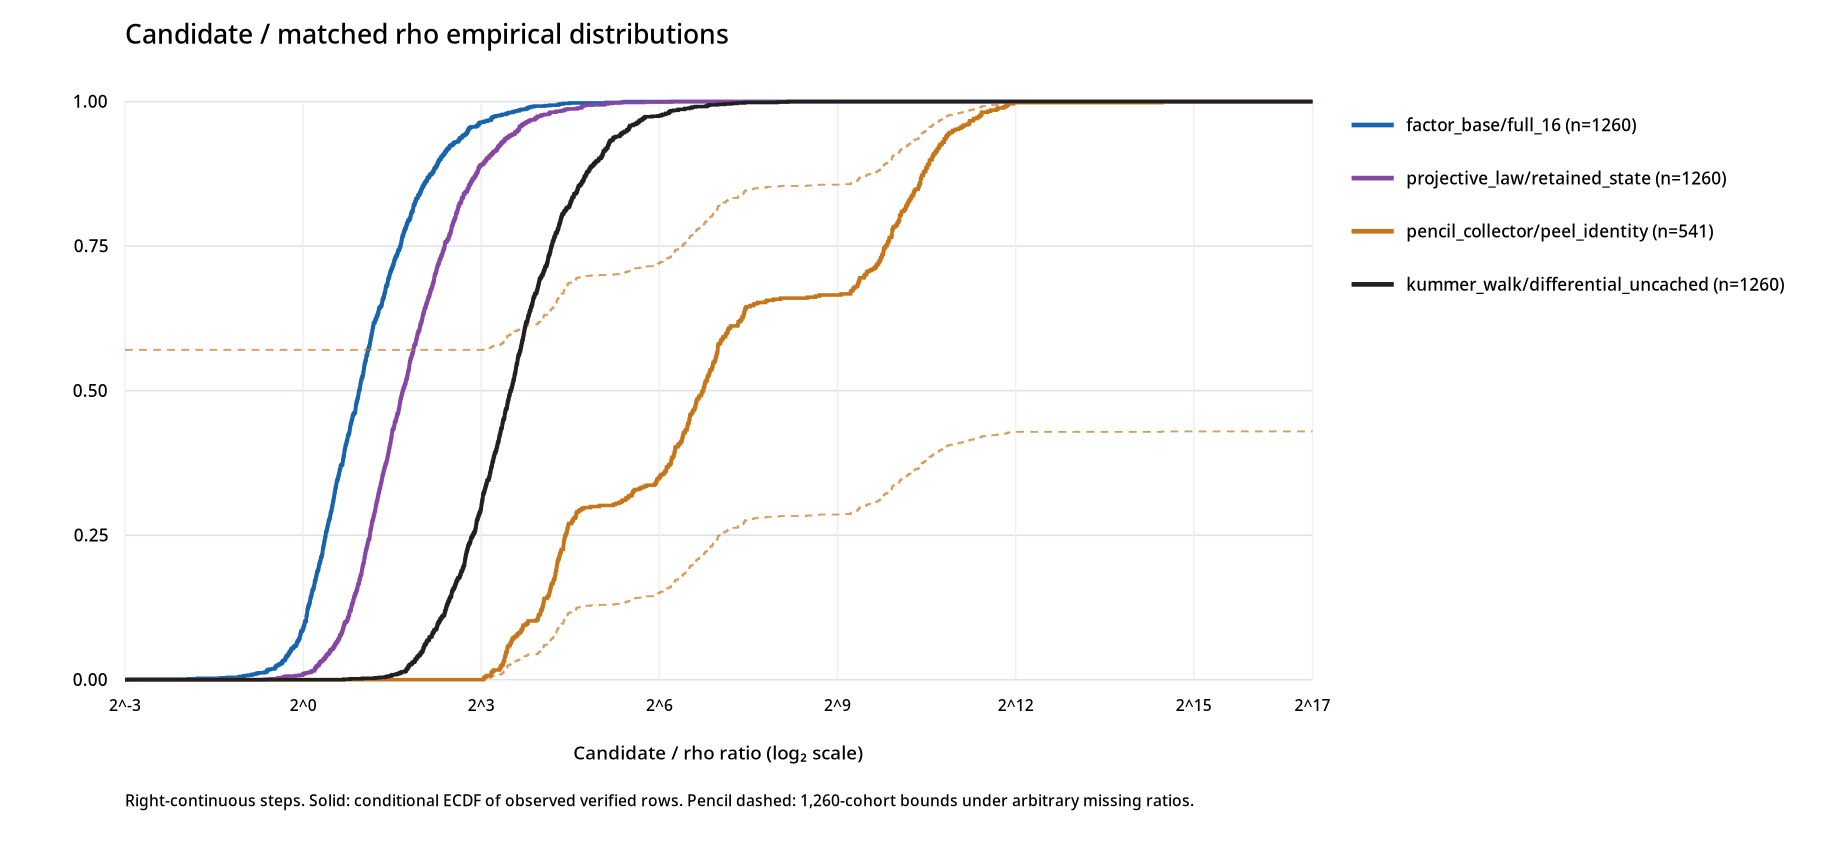
\includegraphics[width=0.98\linewidth]{ecdf.png}
\end{center}

\clearpage
\noindent\textbf{Price sensitivity.} Each panel contains three square prices,
four inversion prices, and three native-logical prices. The factor-base,
projective, and Kummer panels copy complete 1,260-target aggregate rows. The
pencil panel sums candidate and rho costs across its ten observed curve
aggregates before division (541 targets). Numeric labels are candidate/rho
ratios; color is logarithmic across the displayed 144 cells.

\begin{center}
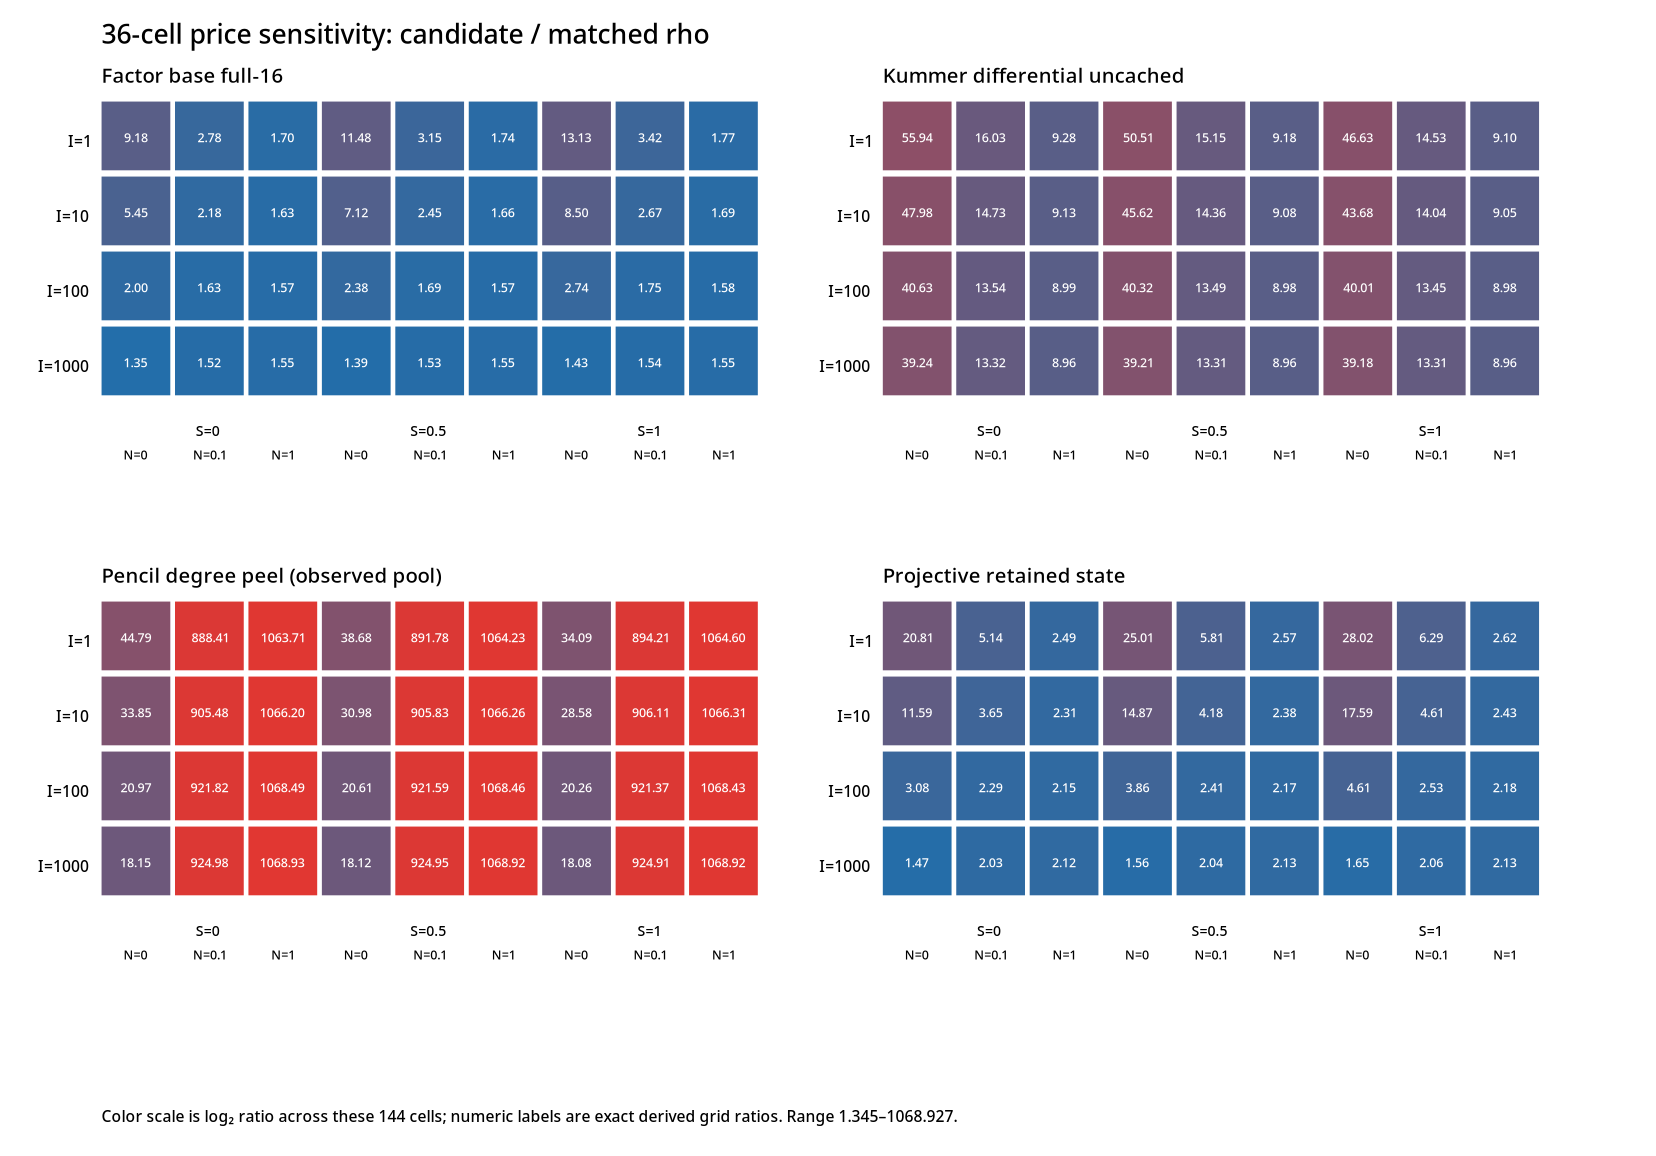
\includegraphics[width=0.98\linewidth]{price-cell-heatmap.png}
\end{center}

\noindent\textbf{Break-even surface.} For every one of 85 complete grid groups,
\path{break-even.csv} reports integer operation-count differences and checks
all 36 cells. With $U=9+4S+I$, equality is
\[
 d_M+d_S S+d_I I+d_L N(9+4S+I)=0.
\]
The maximum per-group absolute and relative reconstruction residuals are
included in the CSV. “Exact” denotes the unique integer coefficients implied
by the 36-cell grid arithmetic; this appendix does not recount source JSON
operation counters. N5 remains partial: phase fractions are absent because the standardized
cross-lead target schema has no common phase-counter columns; no fractions are
inferred from total costs.

\par\medskip
\noindent\textbf{Review files.} \path{paired-deltas.csv} preserves losses,
wins, cap nulls, and coordinate-only exclusions. \path{ecdf.csv} preserves
conditional and cohort-bound values. \path{descriptive-tails.csv} uses
nearest-rank empirical quantiles. \path{cluster-bootstrap.csv} records seeds,
sample sizes, and interval labels. \path{price-cell-heatmap.csv} and
\path{break-even.csv} contain the plotted and algebraic source values.
\end{document}
